%Toy example text
%\todo[inline]{I expect to see first the general control problem 13a-13e, then the specific example. This way, if you define once here, we dnot have to worry about re-defining the control problem later. So: here;s the general control problem; here's a simple system.}

The control problem we solve is a generalized version of \eqref{eq:min rob problem}, using the smooth version of robustness, given by
\begin{subequations}
\label{eq:general_ctrl}
\begin{align}
\text{max } & \srob_{\formula}(\sstraj) - \gamma \sum_{k=0}^{N-1} l(x_{k+1},u_{k}) \\
\text{s.t. } & x_{k+1} = f(x_k,u_k), \, \forall k=0,\dotsc,N-1 \\
 & x_k \in X, \, \forall k=0,\dotsc,N \\
 & u_k \in U, \, \forall k=0,\dotsc,N-1 \\
 & \delta \srob_{\formula}(\sstraj) \geq 0
\end{align}
\end{subequations}
%\todo[inline]{stick to $\formula$ for a formula, not $\formula$ (unless there's a good reason)}

If we set $\gamma=0$ and $\delta=0$, we recover the problem in \eqref{eq:min rob problem} with the smooth robustness in the cost function. In the above formulation, $l(x_{k+1},u_{k})$ is a system specific control cost, e.g. the LQR cost $x_k'Qx_k + u_k'Ru_k$. $X$ and $U$ define constraints on the state $x$ and control $u$ respectively. 

\subsubsection{Illustrative example}
\label{sec:illustrative example}
To illustrate the control algorithm, we choose a simple linear system (point-mass dynamics) to first illustrate our method. The point-mass system has the following dynamics:
\begin{equation}
\label{eq:PointMass}
x_{k+1} = x_k + u_k
\end{equation}

For the point-mass example, the specification is 
\[\formula = \always_{[0,20]} \neg (x_k \in \text{Unsafe}) \land \eventually_{[0,20]} (x_k \in \text{Terminal})\]
with the sets $\text{Unsafe}=[-1,1]^2$ and $\text{Terminal}=[2,2.5]^2$. 
The state space is $X=[-2.5,2.5]^2$, $U=[0.3,0.3]^2$, $\delta=1$, and we optimize for two different values of $\gamma$, $0.1$ and $0.001$.
The initial point of the optimization is $x_0=[-2,-2]'$. 
The control cost is $l(x_k,u_k) = ||x_k||_{2}^2$, so that $\sum_kl(x_k,u_k)$ penalizes the length of the trajectory. Here, $hrz(\formula) = 21$.

An initial trajectory starting from $x_0$ and ending in the $\text{Terminal}$ set is obtained via solving a linear program for feasibility with the system dynamics and input/state constraints, and the terminal set added as a constraint. This trajectory is used as an initial point to initialize the optimization.

We use MATLAB's Sequential Quadratic Programming (SQP) solver for the optimization, and also compute a gradient for $\srob$ to be used in SQP.
%\todo[inline]{confusing...you throw around things casually like $\min 0$, as if you're daring the reader to get confused. Or "This trajectory is used to initialize the SQP optimization, which is used for the optimization."..Take your time. explain it once, well, and then forget about it. this is the \textit{illustrative} example. see my comment in ATC case study.}

\todo[inline]{say a word or two about SQP: broadly, how it works and whether it has guarantees. after all, it is to use things like SQP that we are smoothing in the first place. }

Fig.~\ref{fig:toy control} shows the sets, initial trajectory (which is unsafe and has a robustness of $-1$), and the two trajectories for the two values of $\gamma$. Both trajectories satisfy the specification $\formula$. Intuitively, the trajectories in Fig.\ref{fig:toy control} make sense, as for a higher value of $\gamma=0.1$ we get a shorter trajectory, which is closer to unsafe set, hence satisfies $\formula$ less robustly ($\rob_{\formula}=0.6543$) and for a smaller value of $\gamma=0.001$ we get a longer trajectory which has a higher robustness ($\rob_{\formula}=1.2073$).

\begin{figure}[t]
\centering
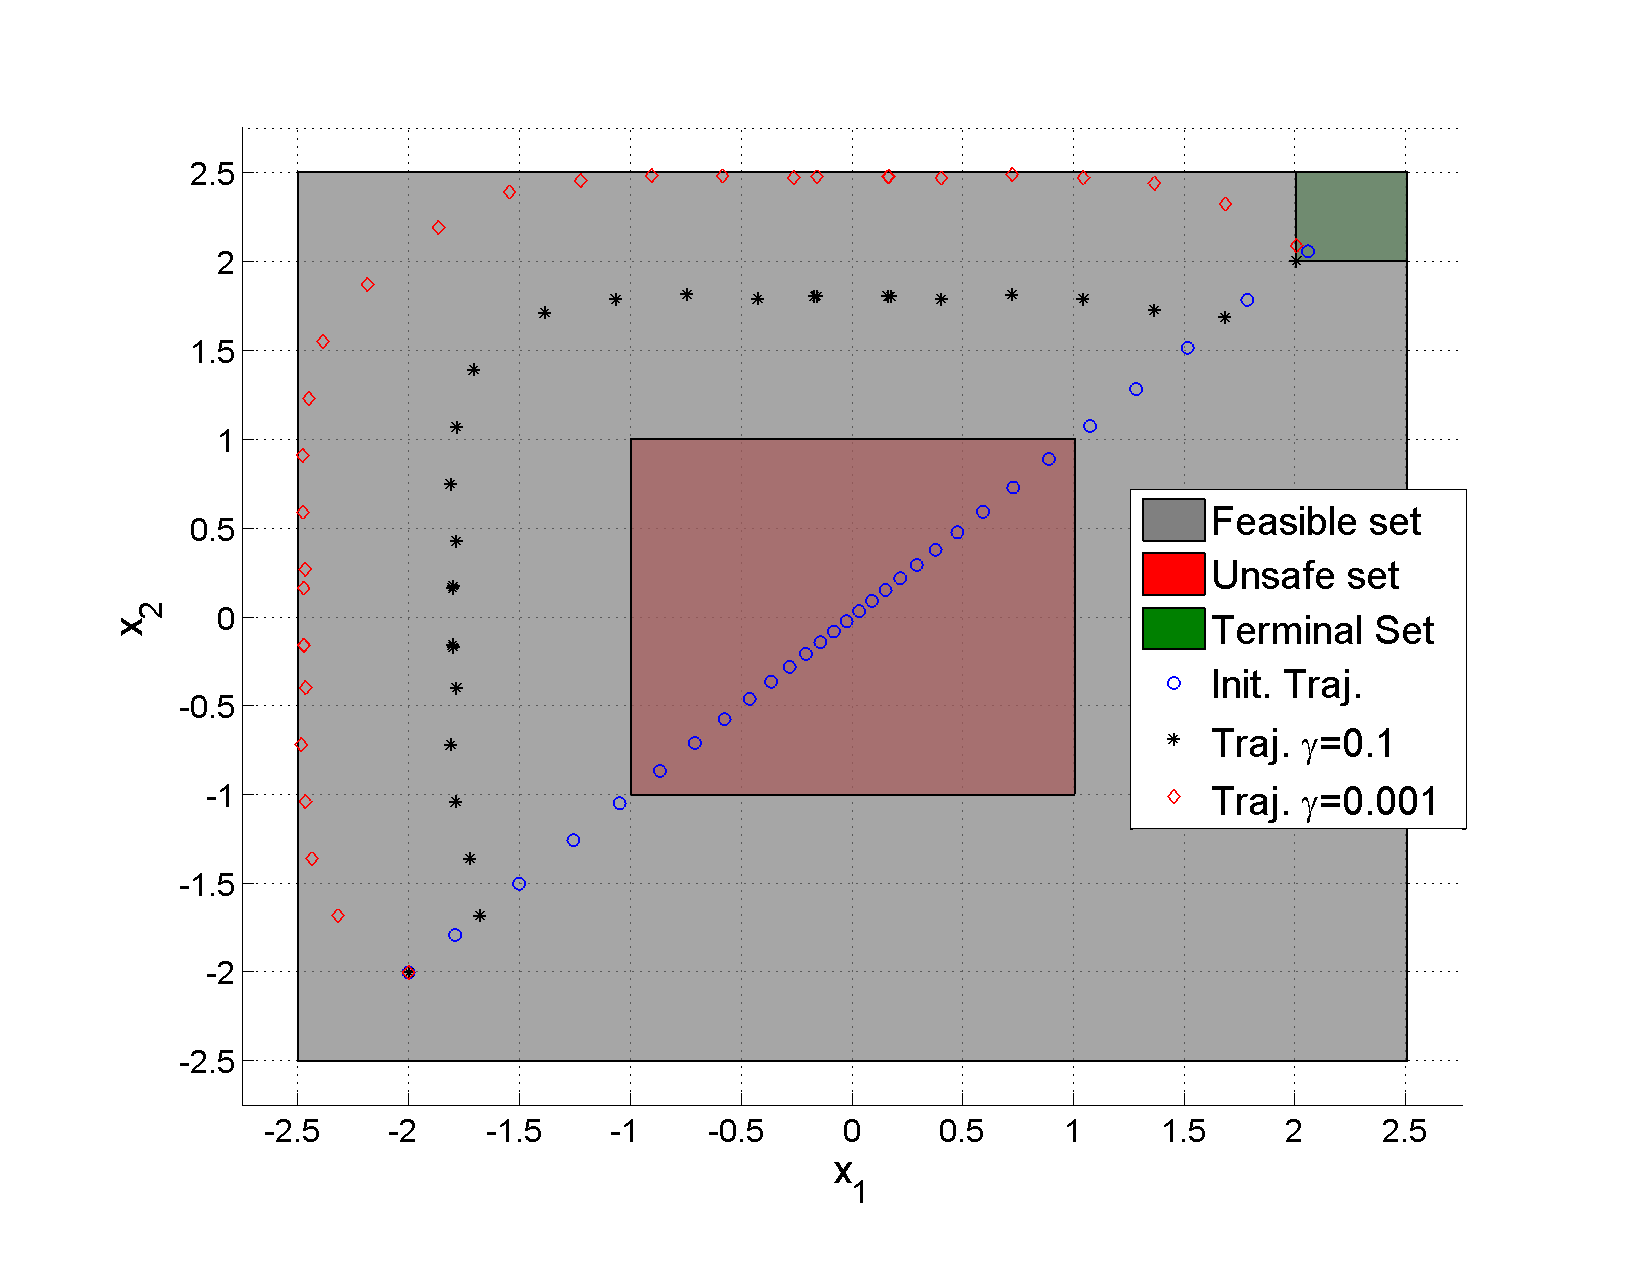
\includegraphics[width=0.49\textwidth]{figures/ToyExampleControl}
\caption{{\small Initial trajectory and trajectories obtained for two different values of $\gamma$ in \eqref{eq:general_ctrl}.}}
\label{fig:toy control}
\end{figure}